\documentclass[final]{beamer}\usepackage[]{graphicx}\usepackage[]{color}
%% maxwidth is the original width if it is less than linewidth
%% otherwise use linewidth (to make sure the graphics do not exceed the margin)
\makeatletter
\def\maxwidth{ %
  \ifdim\Gin@nat@width>\linewidth
    \linewidth
  \else
    \Gin@nat@width
  \fi
}
\makeatother

\definecolor{fgcolor}{rgb}{0.345, 0.345, 0.345}
\newcommand{\hlnum}[1]{\textcolor[rgb]{0.686,0.059,0.569}{#1}}%
\newcommand{\hlstr}[1]{\textcolor[rgb]{0.192,0.494,0.8}{#1}}%
\newcommand{\hlcom}[1]{\textcolor[rgb]{0.678,0.584,0.686}{\textit{#1}}}%
\newcommand{\hlopt}[1]{\textcolor[rgb]{0,0,0}{#1}}%
\newcommand{\hlstd}[1]{\textcolor[rgb]{0.345,0.345,0.345}{#1}}%
\newcommand{\hlkwa}[1]{\textcolor[rgb]{0.161,0.373,0.58}{\textbf{#1}}}%
\newcommand{\hlkwb}[1]{\textcolor[rgb]{0.69,0.353,0.396}{#1}}%
\newcommand{\hlkwc}[1]{\textcolor[rgb]{0.333,0.667,0.333}{#1}}%
\newcommand{\hlkwd}[1]{\textcolor[rgb]{0.737,0.353,0.396}{\textbf{#1}}}%
\let\hlipl\hlkwb

\usepackage{framed}
\makeatletter
\newenvironment{kframe}{%
 \def\at@end@of@kframe{}%
 \ifinner\ifhmode%
  \def\at@end@of@kframe{\end{minipage}}%
  \begin{minipage}{\columnwidth}%
 \fi\fi%
 \def\FrameCommand##1{\hskip\@totalleftmargin \hskip-\fboxsep
 \colorbox{shadecolor}{##1}\hskip-\fboxsep
     % There is no \\@totalrightmargin, so:
     \hskip-\linewidth \hskip-\@totalleftmargin \hskip\columnwidth}%
 \MakeFramed {\advance\hsize-\width
   \@totalleftmargin\z@ \linewidth\hsize
   \@setminipage}}%
 {\par\unskip\endMakeFramed%
 \at@end@of@kframe}
\makeatother

\definecolor{shadecolor}{rgb}{.97, .97, .97}
\definecolor{messagecolor}{rgb}{0, 0, 0}
\definecolor{warningcolor}{rgb}{1, 0, 1}
\definecolor{errorcolor}{rgb}{1, 0, 0}
\newenvironment{knitrout}{}{} % an empty environment to be redefined in TeX

\usepackage{alltt}
\mode<presentation>{\usetheme{confposter}}
\usepackage{amsmath, amsfonts, amssymb, pxfonts, eulervm, xspace, enumerate, hyperref, color, bookmark}

\usepackage{mdframed}
\usepackage{graphicx}
\usepackage[orientation=landscape, size=custom, width =152.4, height=106.68, scale=1.5, debug]{beamerposter}

\setbeamercolor{block title}{fg=black,bg=white} % Colors of the block titles
\setbeamercolor{block body}{fg=black,bg=white} % Colors of the body of blocks
\setbeamercolor{block alerted title}{fg=lgold,bg=black} % Colors of the highlighted block titles
\setbeamercolor{block alerted body}{fg=black,bg=white} % Colors of the body of highlighted blocks
\setbeamercolor{item}{fg=fgreen}
\setbeamercolor{item projected}{fg=white,bg=lgold}
\setbeamercolor{important}{fg=black, bg=lgold}

%\setbeamercolor{background canvas}{bg=white} %setting background color

%optional background below
\setbeamertemplate{background}{
\tikz[overlay,remember picture] \node[opacity=0.3, at=(current page.center)] {
   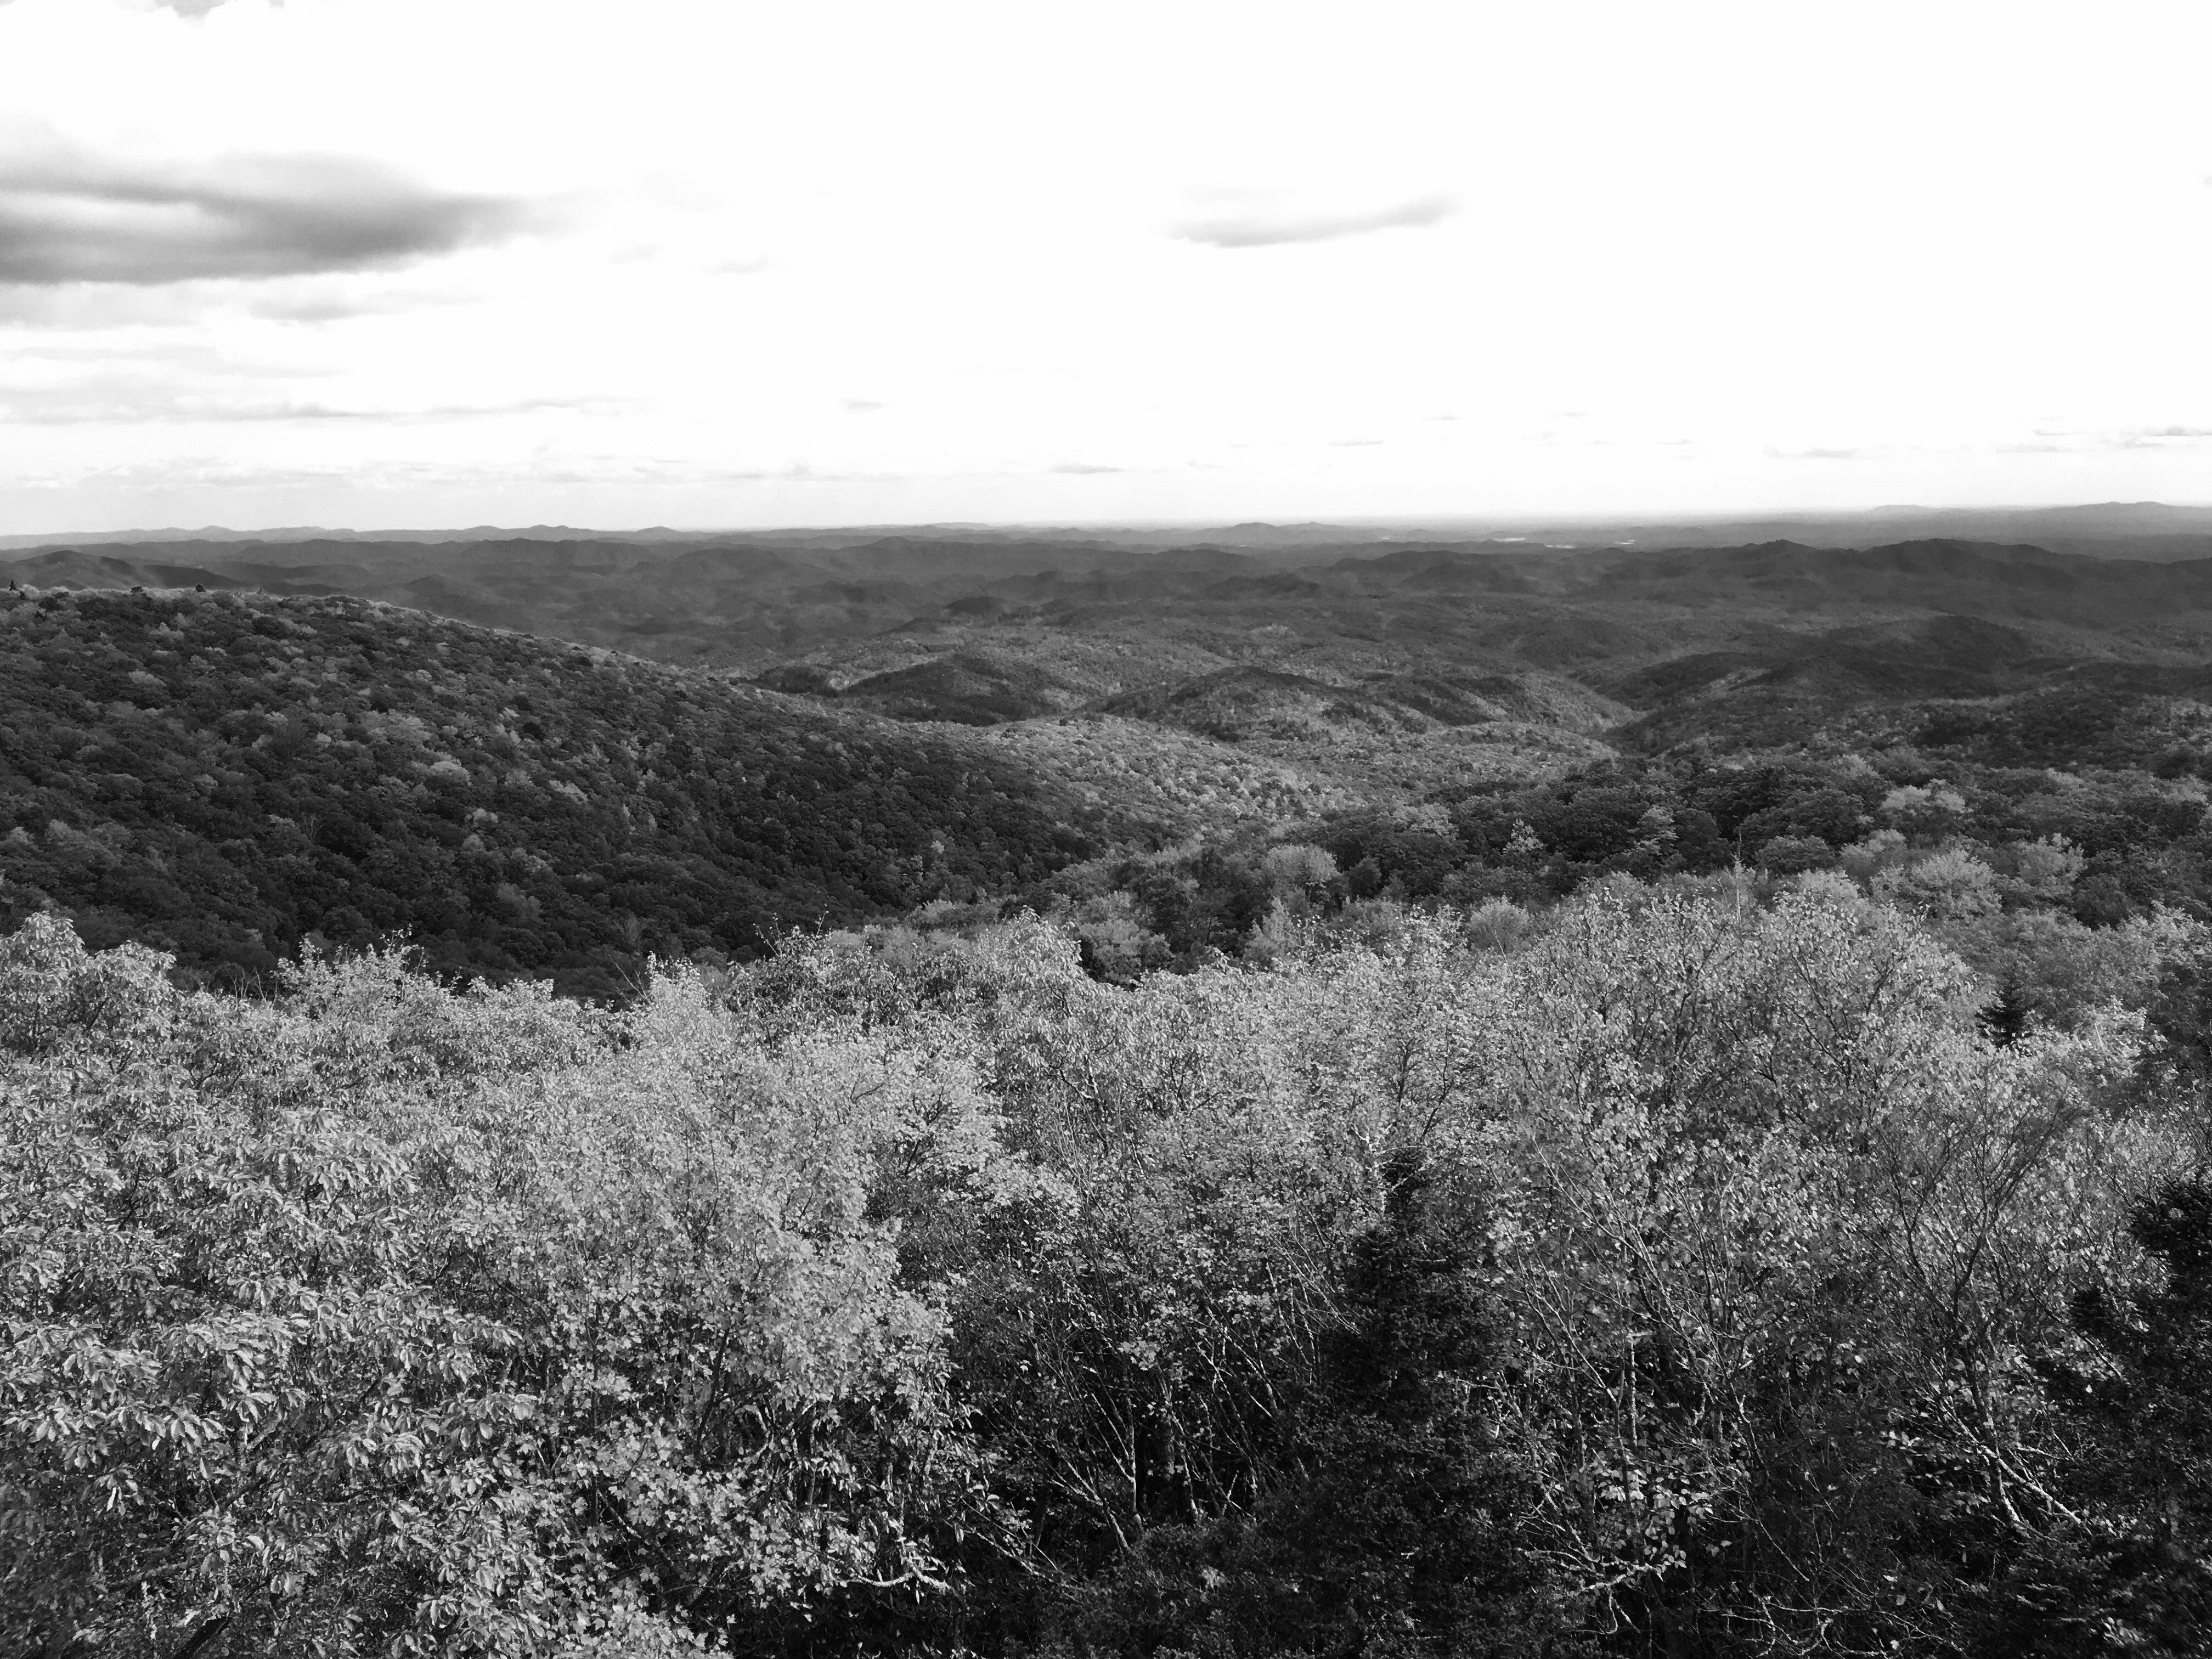
\includegraphics[height=\paperheight,width=\paperwidth]{background.jpg}};
}


%-----------------------------------------------------------
% Define the column widths and overall poster size
% To set effective sepwid, onecolwid and twocolwid values, first choose how many columns you want and how much separation you want between columns
% In this template, the separation width chosen is 0.024 of the paper width and a 4-column layout
% onecolwid should therefore be (1-(# of columns+1)*sepwid)/# of columns e.g. (1-(4+1)*0.024)/4 = 0.22
% Set twocolwid to be (2*onecolwid)+sepwid = 0.464
% Set threecolwid to be (3*onecolwid)+2*sepwid = 0.708

\newlength{\sepwid}
\newlength{\onecolwid}
\newlength{\twocolwid}
\newlength{\threecolwid}
\setlength{\sepwid}{0.024\paperwidth} % Separation width (white space) between columns
\setlength{\onecolwid}{0.22\paperwidth} % Width of one column
\setlength{\twocolwid}{0.464\paperwidth} % Width of two columns
\setlength{\threecolwid}{0.708\paperwidth} % Width of three columns
\setlength{\topmargin}{-0.5in} % Reduce the top margin size
%-----------------------------------------------------------

\usepackage{graphicx}  % Required for including images

\usepackage{booktabs} % Top and bottom rules for tables

%----------------------------------------------------------------------------------------
%	TITLE SECTION 
%----------------------------------------------------------------------------------------

\title{Analyzing and Influencing Carbon Sequestration in Harvested Wood Products} % Poster title

\author{Alan Arnholt, Ben Jones, Hannah X Laws, Kelly Loucks, Eric Marland, Andrew Sullivan} % Author(s)

\institute{Department of Mathematical Sciences} % Institution(s)

%----------------------------------------------------------------------------------------
\IfFileExists{upquote.sty}{\usepackage{upquote}}{}
\begin{document}

\addtobeamertemplate{block end}{}{\vspace*{2ex}} % White space under blocks
\addtobeamertemplate{block alerted end}{}{\vspace*{2ex}} % White space under highlighted (alert) blocks


\setlength{\belowcaptionskip}{2ex} % White space under figures
\setlength\belowdisplayshortskip{2ex} % White space under equations

\begin{frame}[t] % The whole poster is enclosed in one beamer frame

%logos in title section
\begin{tikzpicture}[remember picture,overlay]
%add logos in corners
\node[anchor=north west] at ([shift={(6cm,0cm)}]current page.north west)
    {
\includegraphics[width=9cm]{usfs.png}};
\node[anchor=north east] at ([shift={(-3cm,-1cm)}]current page.north east)
    {
\includegraphics[width=23cm]{app.png}};
\end{tikzpicture}

\begin{columns}[t] % The whole poster consists of three major columns, the second of which is split into two columns twice - the [t] option aligns each column's content to the top

\begin{column}{\sepwid}\end{column} % Empty spacer column

\begin{column}{\onecolwid} % The first column

%----------------------------------------------------------------------------------------
%	OBJECTIVES
%----------------------------------------------------------------------------------------
%Abstract
%----------------------------------------------------------------------------------------

%changing color             
\setbeamercolor{block alerted title}{fg=lgold,bg=black} % Change the alert block title colors
\setbeamercolor{block alerted body}{fg=black,bg=white} % Change the alert block body colors
\setbeamercolor{item}{fg=lgold, bg=black}

\begin{alertblock}{Abstract}
\begin{tikzpicture}[remember picture,overlay]
      \shade [inner color=silver,outer color=lgold]
      (0,0) rectangle (\textwidth,0.4cm);
    \end{tikzpicture}

WOODCARB3 expands the capabilities of the WOODCARB2 spreadsheet model by changing to an R package platform. The conversion brings increased capability for data manipulation, analysis, and reporting. It also increases the ease of integration with other datasets. This poster describes some of the results and demonstrates some of the potential for the WOODCARB3 model. Examples of the types of analysis possible include uncertainty analysis, sensitivity analysis, alternate model dynamics, alternate pathways.

\vspace{0ex}

\end{alertblock}
%-------------------------------------------------------------
\begin{block}{Introduction}


WOODCARB2 is used to document and calculate the total carbon stocks from harvested wood products (HWP). The statistics package R offers a wide variety of tools and interfaces with other software packages.
\vspace{1ex}

Sequestration of carbon in forests accounts for 87\% of total \textbf{CO$_{2}$} removals in 2014. Carbon mitigation efforts have thus focused much attention on reforestation, forest management,and forest based products. According to the most recent report to the \textbf{UNFCCC}, an estimated 18.7\% of the total carbon in woody materials is contained in harvested wood \textbf{(HWP and SWDS).}
\vspace{1ex}  

The amount of carbon in \textbf{HWP} and \textbf{SWDS} depend on how much wood is harvested, what types of products are produced, how the products are use, the lifetime of the wood products, and how the wood is processed at the end of its primary product lifetime.



\end{block}


%------------------------------------------------
\setbeamercolor{block title}{fg=black,bg=white}
\begin{block}{Sources of Data and Equations}

\begin{enumerate}[I.]
\item Input data from reports by Hair, Ulrich, Howard, Ince, etc. 
\vspace{.3ex}
\item The Production Approach is:  
\begin{equation}
\frac{44}{12} * \Big(-\Delta C_{HWP\:IU\:DH} - \Delta C_{HWP\:SWDS\:DH}\Big)
\label{eqn:Einstein}
\end{equation}
\vspace{.3ex}
\item $\frac{44}{12}$ converts Carbon to $CO_2$
\vspace{.3ex}
\item $\Delta C_{HWP\:IU\:DH}$ is change in stock of HWP in use from 
domestic harvest 
\vspace{.3ex}
\item $\Delta C_{HWP\:SWDS\:DH}$ is change in stock of HWP in SWDS
from domestic harvest 
\end{enumerate}
\vspace{.3ex}
\end{block}
\vfill

%----------------------------------------------------------------------------------------
% Methodology
%----------------------------------------------------------------------------------------
\setbeamercolor{block title}{fg=fgreen,bg=white}
\begin{block}{Methodology}
\begin{itemize}
\item Most analysis done with the Production approach.
\vspace{.5ex}
\item The Production approach focuses on carbon stocks in wood harvested in the US.
\vspace{.5ex}
\item Analysis is conducted of sensitivity of input parameters, uncertainty of estimates
and consequences of alternative decay distributions. 
\end{itemize}
\vspace{.3ex}
\vfill
\end{block}
%----------------------------------------------------------------------------------------

\end{column} % End of the first column

\begin{column}{\sepwid}\end{column} % Empty spacer column

\begin{column}{\twocolwid} % Begin a column which is two columns wide (column 2)

\begin{columns}[t,totalwidth=\twocolwid] % Split up the two columns wide column

\begin{column}{\onecolwid}\vspace{-.6in} % The first column within column 2 (column 2.1)

%----------------------------------------------------------------------------------------
%	PURPOSE
%----------------------------------------------------------------------------------------

%changing color             
\setbeamercolor{block title}{fg=black,bg=black} % Change the alert block title colors
\setbeamercolor{block body}{fg=black,bg=white} % Change the alert block body colors
\setbeamercolor{item}{fg=lgold, bg=black}

\begin{block}{Uncertainty Analysis}
\begin{tikzpicture}[remember picture,overlay]
      \shade [inner color=silver,outer color=lgold]
      (0,0) rectangle (\textwidth,0.4cm);
    \end{tikzpicture}
\begin{itemize}
\item Information is intended to aid in international discussions and any agreements about managing greenhouse gas emissions and sinks.
\item Also provides national level methods and estimates of carbon sinks and emissions associated with HWP.
\item The package provides quick accessibility, allowing data to be updated, modified, and manipulated with ease.
\end{itemize}
\end{block}



%----------------------------------------------------------------------------------------

\end{column} % End of column 2.1

\begin{column}{\onecolwid}\vspace{-.6in} % The second column within column 2 (column 2.2)

%----------------------------------------------------------------------------------------
%	Plot
%----------------------------------------------------------------------------------------
\setbeamercolor{block title}{fg=black,bg=white}
\setbeamercolor{block body}{fg=black,bg=white}
\begin{block}{Projected Carbon Contribution}
\begin{figure}
    {\includegraphics[width=1\linewidth,height=11cm]{projection.png}};
\end{figure}
{\bf Figure 1:} Projected carbon contribution based on five and ten year regressed projections.
\end{block}

%----------------------------------------------------------------------------------------

\end{column} % End of column 2.2

\end{columns} % End of the split of column 2 - any content after this will now take up 2 columns width

%----------------------------------------------------------------------------------------
%	IMPORTANT RESULT
%----------------------------------------------------------------------------------------

\begin{alertblock}{Total HWP Carbon Stocks with Uncertainty}
\begin{center}

\begin{figure}
    {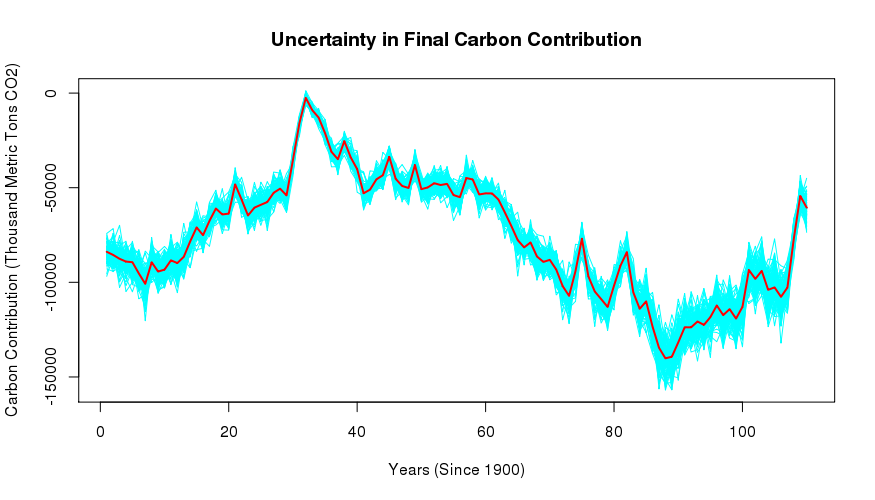
\includegraphics[width=1\linewidth,height=10cm]{Uncertainty_Plot.png}};
    \caption{this is the caption that shows what is in the figure that explains the plot of HWP stocks and provides and envelope of uncertainty around it
    this is the caption that shows what is in the figure that explains the plot of HWP stocks and provides and envelope of uncertainty around it}
\end{figure}
\end{center}
\end{alertblock} 

%----------------------------------------------------------------------------------------

\begin{columns}[t,totalwidth=\twocolwid] % Split up the two columns wide column again

\begin{column}{\onecolwid} % The first column within column 2 (column 2.1)

\setbeamercolor{block title}{fg=black,bg=black} % Change the alert block title colors
\setbeamercolor{block body}{fg=black,bg=white} % Change the alert block body colors
\setbeamercolor{item}{fg=lgold, bg=black}

\begin{block}{Decay}
\begin{itemize}
\item Decay functions are based on the gamma distribution:
$$\int_{0}^{n}\frac{1}{\Gamma(k)\theta(k)}x^{k-1}e^{-x/k}dx$$
\item WOODCARB2 used an exponential decay where $k=1$ in the gamma distribution
\item Two alternate decay functions, $k=2$ and $k=10$, were calculated by altering $k$ in the gamma distribution and introduced in the WOODCARB3R package
\end{itemize}
\end{block}
%----------------------------------------------------------------------------------------
\begin{block}{Decay of Hardwood in Multifamily housing}
\begin{center}
\begin{figure}
    {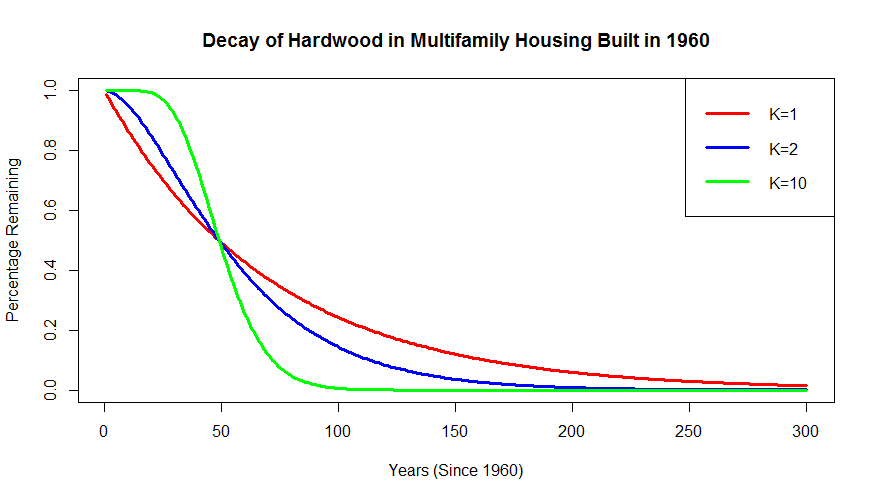
\includegraphics[width=1\linewidth, height=9cm]{Decay_Plot_Example.png}};
    \caption{This figure shows the over effect of the decay function on multifamily housing built in 1960}
\end{figure}
\end{center}

\end{block}


%----------------------------------------------------------------------------------------

\end{column} % End of column 2.1

\begin{column}{\onecolwid} % The second column within column 2 (column 2.2)

%----------------------------------------------------------------------------------------


%----------------------------------------------------------------------------------------

%Half Life Table
%-----------------------------------------------------------------------------

\begin{block}{Halflife Table}
\begin{center}
\begin{figure}
{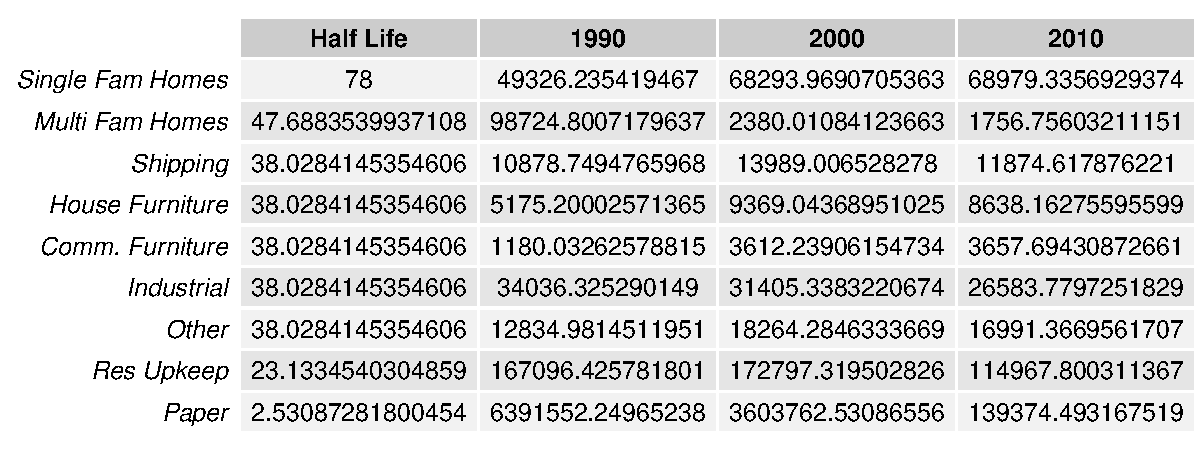
\includegraphics[width=1\linewidth, height=17cm]{CopyOfHLTable.pdf}}
      \caption{Figure caption}
  \end{figure}
  \end{center}
  \end{block}

%----------------------------------------------------------------------------------------
\begin{block}{Overall Decay}
\begin{center}
\begin{figure}
    {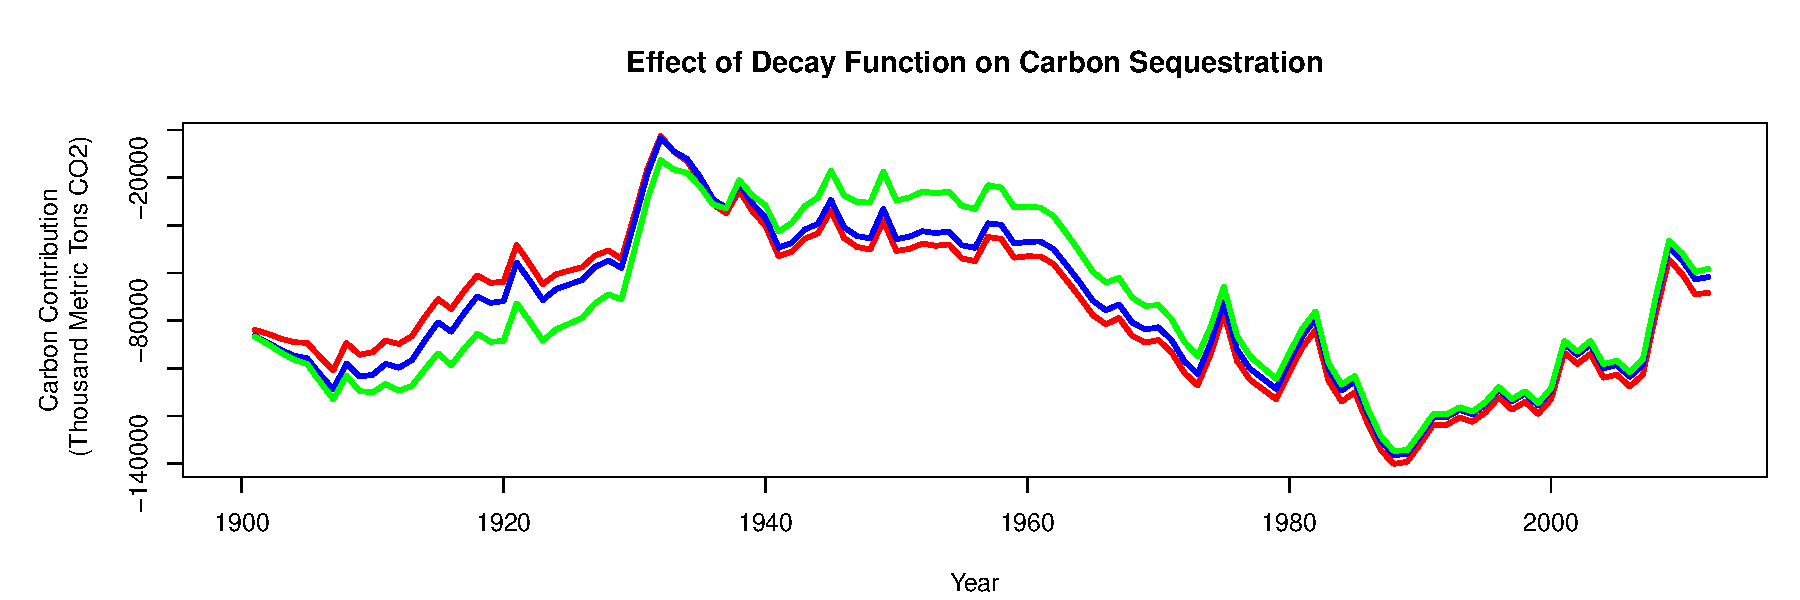
\includegraphics[width=1\linewidth, height=9cm]{DecayPlotOverall.pdf}};
    \caption{This figure shows the over effect of the decay function on Carbon Sequestration}
\end{figure}
\end{center}

\end{block}
%---------------------------------------------------------------------


\end{column} % End of column 2.2

\end{columns} % End of the split of column 2

\end{column} % End of the second column

\begin{column}{\sepwid}\end{column} % Empty spacer column

\begin{column}{\onecolwid} % The third column

%----------------------------------------------------------------------------------------
\setbeamercolor{block title}{fg=black,bg=black} % Change the alert block title colors
\setbeamercolor{block body}{fg=black,bg=white} % Change the alert block body colors
\setbeamercolor{item}{fg=lgold, bg=black}

\begin{block}{Sensitivity Analysis}
\begin{itemize}
\item Information is intended to aid in international discussions and any agreements about managing greenhouse gas emissions and sinks.
\item Also provides national level methods and estimates of carbon sinks and emissions associated with HWP.
\item 
\end{itemize}
\vspace{0ex}

\end{block}
%----------------------------------------------------------------------------------------
%	Sensitivity Plot
%----------------------------------------------------------------------------------------

\begin{block}{Sensitivity Plot}
\begin{center}
\begin{figure}
    {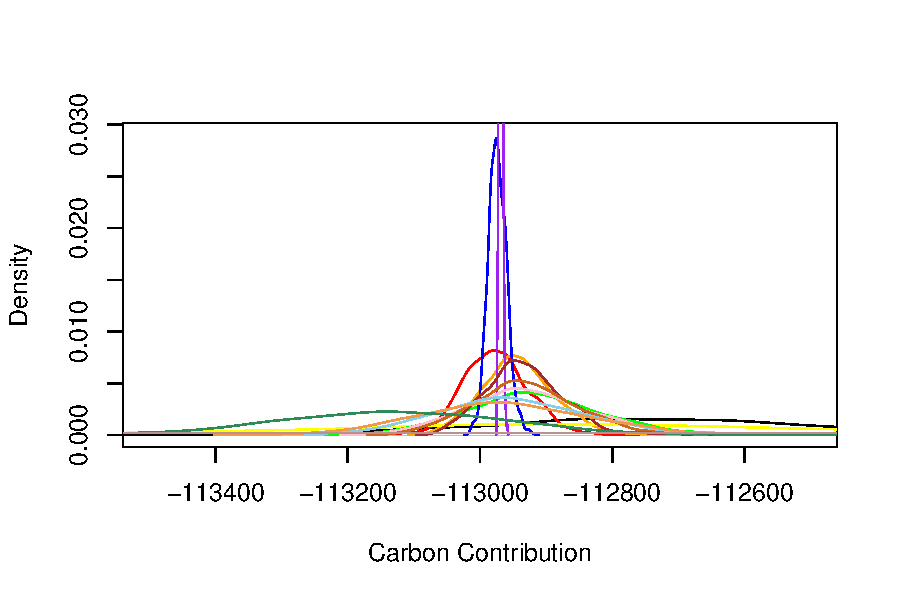
\includegraphics[width=1\linewidth,height=10cm]{CopyOfHLSensitivityGraph.pdf}};
    \caption{Figure caption}
\end{figure}
\end{center}
\end{block}


%----------------------------------------------------------------------------------------
%	Discussion
%----------------------------------------------------------------------------------------

\begin{block}{Discussion}

\begin{itemize}
\item Targeted changes in average half life can increase total stocks.
\item End of life dynamics make a big difference in stock size.
\item Sensitivities help channel reductions in uncertainty.
\end{itemize}

\end{block}



%----------------------------------------------------------------------------------------
%	ACKNOWLEDGEMENTS
%----------------------------------------------------------------------------------------

\setbeamercolor{block title}{fg=fgreen,bg=white} % Change the block title color

\begin{block}{Acknowledgements}

This work was funded by a Research Joint Venture Agreements with the USDA Forest Service, Northern Research Station and the USDA Forest Service, Southern Research Station.

\end{block}

%----------------------------------------------------------------------------------------
%	CONTACT INFORMATION
%----------------------------------------------------------------------------------------

\setbeamercolor{block alerted title}{fg=lgold,bg=black} % Change the alert block title colors
\setbeamercolor{block alerted body}{fg=black,bg=white} % Change the alert block body colors

\begin{alertblock}{Contact Information and Package Access}

\begin{itemize}
\item Email: \href{marlandes@appstate.edu}{marlandes@appstate.edu}
\item Online link: \href{http://benjones2.github.io/WOODCARB3R/}{WOODCARB3R package}
%qr code below
\end{itemize}
\vspace{0ex}
\begin{center}
\begin{tikzpicture}
\node[anchor=south west] at ([shift={(0cm,0cm)}]current page.south west)
  {
\includegraphics[width=8cm]{qrcode.jpg}};
\end{tikzpicture}
\end{center}

\end{alertblock}

%-----------------------------------------------------------------------------

%----------------------------------------------------------------------------------------

\end{column} % End of the third column

\end{columns} % End of all the columns in the poster

\end{frame} % End of the enclosing frame

\end{document}

